\documentclass[12pt]{article}
\usepackage[utf8]{inputenc}
\usepackage[T2A]{fontenc}
\usepackage[mongolian]{babel}
\usepackage{graphicx}
\begin{document}
	\section{Хэрэглэгчийн функциональ шаардлага} 
	\begin{itemize}		 
	\item Шэйр хийсэн файлаа устгаж болно
	\item Тайлбар бичиж болно
	\item Засаж болно
	\item Устгаж болно
	\item Бусад найзтай таг хийж болно
	\item Тахиргоо хийж болно (нийтлэг, найз, өөрөө)
	\item  Шэйр хийсэн цагаа харж болно.
	\item Бусад хүмүүс шэйр хийж болно  
	\item Группын файл бол админ нь устгаж болно
\section{Хэрэглэгчийн функциональ бус шаардлага}
	\item Олон хэрэглэгч шейр хийх боломжтой. 
	\item Хялбар хурдан байх.

	\section{Юзкейс диаграм}
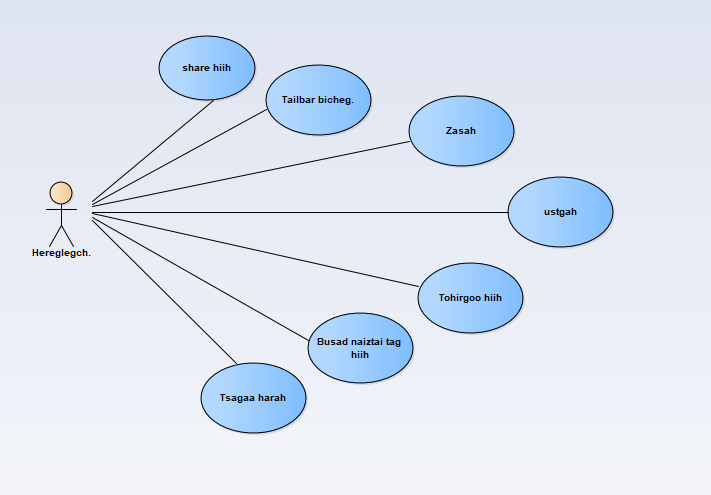
\includegraphics[scale=0.80]{image/usecase.PNG}
    \section{Үйл ажиллгааны  диаграм}
    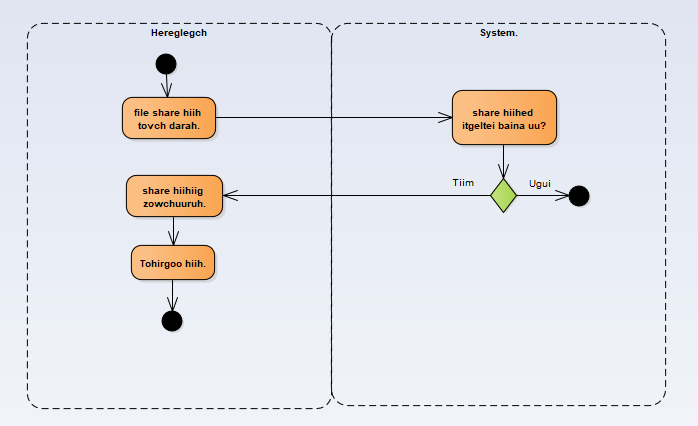
\includegraphics[scale=0.80]{image/Activity_diagram.PNG}
    \section{ER диаграм}
    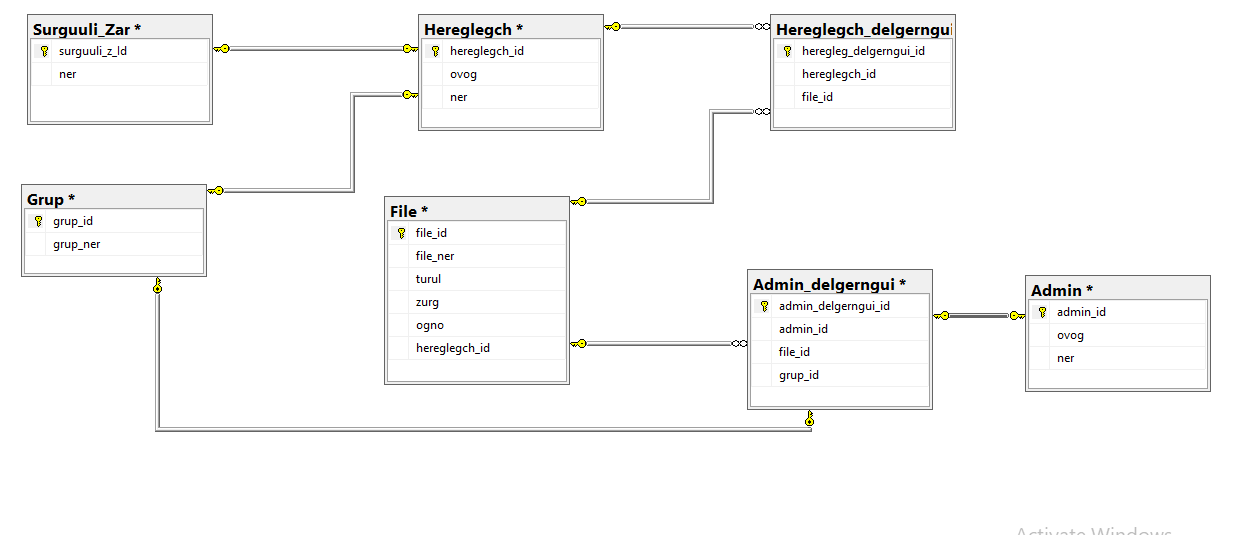
\includegraphics[scale=0.50]{image/ERdiagram.PNG}
    \section{Класс диаграм}
    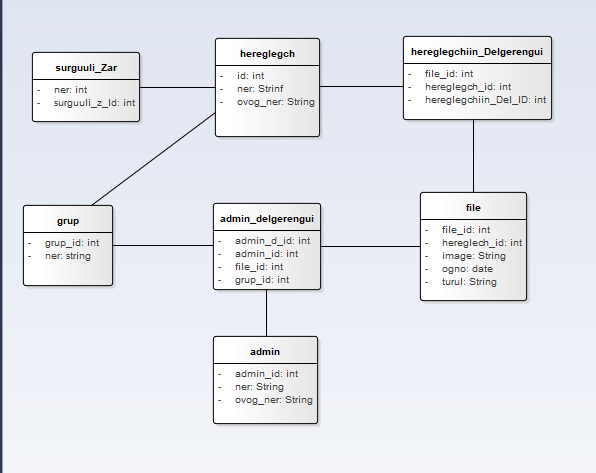
\includegraphics[scale=0.80]{image/class.PNG}
    \section{Дарааллын диаграм}
    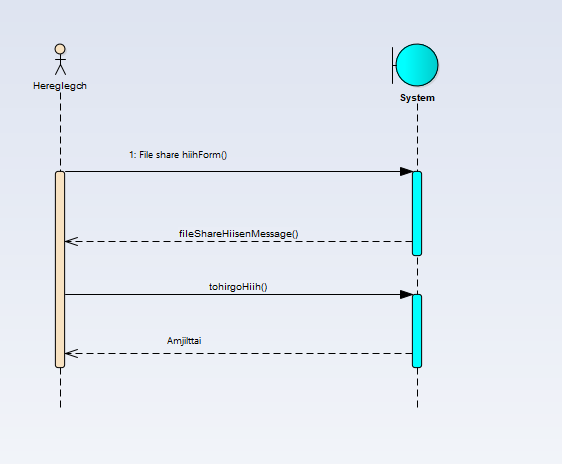
\includegraphics[scale=0.80]{image/seq.PNG}
\end{itemize}
\end{document}
